\documentclass[tikz,border=5pt]{standalone}
\usepackage[T1]{fontenc}
\usepackage{lmodern}
\usepackage{xcolor}
\usetikzlibrary{arrows.meta,positioning}

\definecolor{ink}{HTML}{17233B}
\definecolor{blue}{HTML}{2F6FED}
\definecolor{bluefill}{HTML}{EAF1FF}
\definecolor{teal}{HTML}{157A75}
\definecolor{tealfill}{HTML}{E8F6F4}
\definecolor{red}{HTML}{A33A3A}
\definecolor{redfill}{HTML}{FBECEC}
\definecolor{grayfill}{HTML}{F2F4F8}

\begin{document}
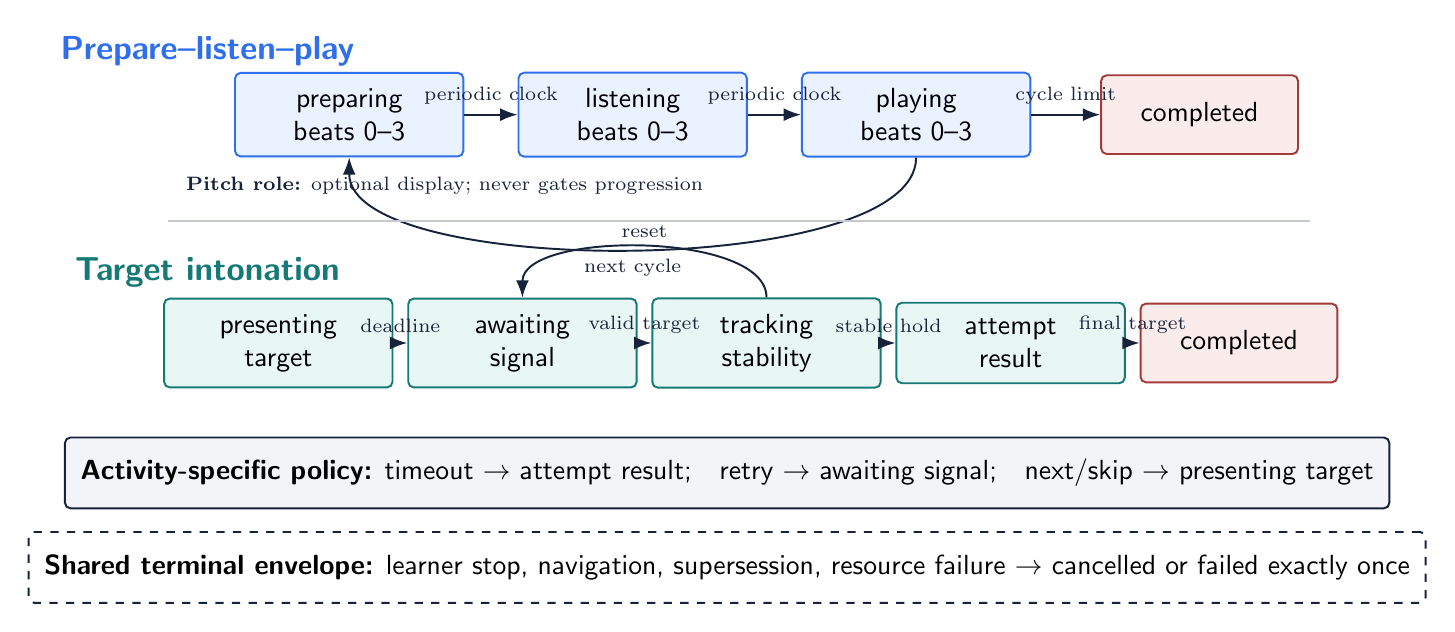
\begin{tikzpicture}[
  font=\sffamily,
  line width=.7pt,
  >={Latex[length=2.2mm]},
  state/.style={draw=ink, rounded corners=2pt, align=center,
    minimum height=10mm, minimum width=29mm, inner sep=2mm},
  plp/.style={state, draw=blue, fill=bluefill},
  ti/.style={state, draw=teal, fill=tealfill},
  terminal/.style={state, draw=red, fill=redfill, minimum width=25mm},
  arrow/.style={->, draw=ink},
  note/.style={font=\scriptsize, text=ink, align=center}
]

\node[font=\sffamily\bfseries\large, text=blue] at (-6.6,.8)
  {Prepare--listen--play};
\node[plp] (prep) at (-4.8,0) {preparing\\beats 0--3};
\node[plp] (listen) at (-1.2,0) {listening\\beats 0--3};
\node[plp] (play) at (2.4,0) {playing\\beats 0--3};
\node[terminal] (plpend) at (6.0,0) {completed};

\draw[arrow] (prep) -- node[note,above] {periodic clock} (listen);
\draw[arrow] (listen) -- node[note,above] {periodic clock} (play);
\draw[arrow] (play) -- node[note,above] {cycle limit} (plpend);
\draw[arrow] (play.south) to[out=-90,in=-90,looseness=.55]
  node[note,below] {next cycle} (prep.south);
\node[note, anchor=west] at (-7.0,-.9)
  {\textbf{Pitch role:} optional display; never gates progression};

\draw[ink!25, line width=.5pt] (-7.1,-1.35) -- (7.4,-1.35);

\node[font=\sffamily\bfseries\large, text=teal] at (-6.6,-2.0)
  {Target intonation};
\node[ti] (present) at (-5.7,-2.9) {presenting\\target};
\node[ti] (await) at (-2.6,-2.9) {awaiting\\signal};
\node[ti] (tracking) at (.5,-2.9) {tracking\\stability};
\node[ti] (result) at (3.6,-2.9) {attempt\\result};
\node[terminal] (tiend) at (6.5,-2.9) {completed};

\draw[arrow] (present) -- node[note,above] {deadline} (await);
\draw[arrow] (await) -- node[note,above] {valid target} (tracking);
\draw[arrow] (tracking) -- node[note,above] {stable hold} (result);
\draw[arrow] (result) -- node[note,above] {final target} (tiend);
\draw[arrow] (tracking.north) to[out=90,in=90,looseness=.7]
  node[note,above] {reset} (await.north);
\node[state, draw=ink, fill=grayfill, minimum width=138mm,
  minimum height=9mm] at (0,-4.55)
  {\textbf{Activity-specific policy:}
   timeout $\rightarrow$ attempt result;\quad
   retry $\rightarrow$ awaiting signal;\quad
   next/skip $\rightarrow$ presenting target};

\node[state, draw=ink, dashed, fill=white, minimum width=138mm,
  minimum height=9mm] at (0,-5.75)
  {\textbf{Shared terminal envelope:}
   learner stop, navigation, supersession, resource failure
   $\rightarrow$ cancelled or failed exactly once};

\end{tikzpicture}
\end{document}
